% ============================================================================
%  Relativistic formulation of the Information Tension field:
%  unifying galactic dynamics, gravitational lensing, and cosmic structure
%
%  R. W. Yett
%  Target: Physical Review D / JCAP
%  Compiled with pdflatex
% ============================================================================
\documentclass[twocolumn,amsmath,amssymb,floatfix]{article}

\usepackage{amsmath,amssymb,amsfonts}
\usepackage{graphicx}
\usepackage{xcolor}
\usepackage{natbib}
\usepackage{booktabs}
\usepackage{hyperref}
\usepackage{geometry}

\geometry{
  letterpaper,
  left=1.8cm, right=1.8cm,
  top=2.2cm, bottom=2.2cm,
  columnsep=0.6cm
}

\hypersetup{
  colorlinks=true,
  linkcolor=blue!60!black,
  citecolor=blue!60!black,
  urlcolor=blue!60!black
}

\newcommand{\lcdm}{\ensuremath{\Lambda}CDM}
\newcommand{\msq}{\ensuremath{\,\mathrm{m\,s^{-2}}}}
\newcommand{\gmunu}{g_{\mu\nu}}
\newcommand{\tmunu}{\tilde{g}_{\mu\nu}}

\bibliographystyle{JHEP}

\begin{document}

\title{Relativistic formulation of the Information Tension field:\\
unifying galactic dynamics, large-scale structure, and dark energy\\
from the Stiefel manifold vacuum}

\author{Ryan W.\ Yett}
\date{%
  \small Chyren Sovereign Intelligence, Independent Research\\
  \small ORCID: 0009-0001-1303-7190\\
  \small \texttt{ryan.yett@chyren.io}\\[6pt]
  \small\today
}

\maketitle

\begin{abstract}
We present a fully covariant formulation of the Information Tension framework, establishing a complete unification of the cosmological Dark Sector (Dark Matter, Dark Energy, and galactic acceleration) from fundamental geometry. Building on the derivation of the acceleration scale $a_0 = c H_0 / 2\pi$ from the Stiefel-manifold bound $\chi = 1/\sqrt{2}$, we elevate the framework to a relativistic scalar-vector-tensor theory. We demonstrate that ordinary baryonic matter couples to these geometric fields via a disformal metric, resolving the historical tension between modified gravity and Bullet Cluster lensing. In the early Universe, rapid oscillations of the massive $\chi$ field act macroscopically as a pressureless fluid ($\langle c_s^2 \rangle \approx 0$), seeding the Cosmic Microwave Background (CMB) acoustic peaks. At late times, Hubble friction freezes the field at its topological bound $\chi_0 = 1/\sqrt{2} \approx 0.707$. We reveal that this geometric resting state not only locks in the MOND acceleration scale but predicts a value of $\Omega_{\text{tension}} = 1/\sqrt{2} \approx 0.707$ in excellent agreement with the observed Dark Energy density fraction ($\Omega_\Lambda \approx 0.69 - 0.71$). The entire Dark Sector is thus eliminated, replaced by the vacuum topological constraints of the Stiefel manifold.
\end{abstract}

% ============================================================================
\section{Introduction}

The cosmological standard model (\lcdm) relies on non-baryonic cold dark matter to explain the formation of large-scale structure, the acoustic peaks of the Cosmic Microwave Background (CMB), and the gravitational lensing of galaxy clusters \citep{Planck2020, Bertone2018}. However, on galactic scales, the dynamics of rotating disks are governed by an incredibly tight correlation between observed acceleration and baryonic acceleration: the Radial Acceleration Relation (RAR) \citep{McGaugh2016}. This relation is phenomenologically codified by Modified Newtonian Dynamics (MOND) \citep{Milgrom1983, Famaey2012}, which introduces a universal acceleration scale $a_0 \approx 1.2 \times 10^{-10}\msq$.

Recently, it was shown that this acceleration scale is not an empirical free parameter, but a geometric necessity. The cosmological acceleration floor derives from the alignment bound of a gauge field on the Stiefel manifold $V_2(\mathbb{R}^4)$, yielding $a_0 = c H_0 / 2\pi \approx 1.04 \times 10^{-10}\msq$, which provides a parameter-free geometric derivation of $a_0$ that fits the SPARC database with competitive accuracy.

However, pure MOND is a non-relativistic modification of Poisson's equation. It fails to account for gravitational lensing \citep{Clowe2006} and lacks the fluid-like behavior necessary to seed the CMB's third acoustic peak. Previous attempts to relativize MOND, such as Bekenstein's Tensor-Vector-Scalar (TeVeS) theory \citep{Bekenstein2004} or the recent Aether-Scalar-Tensor (AeST) theory \citep{Skordis2021}, required positing novel fields in an ad-hoc manner to fit the data.

In this paper, we demonstrate that the required fields are already explicitly present in the geometric derivation of $a_0$. We construct the complete Relativistic Information Tension action, proving that the geometry that fixes galactic dynamics also fundamentally solves lensing and early-universe structure formation.

% ============================================================================
\section{The Relativistic Action}

\subsection{Fields from the Stiefel Manifold}

The vacuum geometry is described by the Stiefel manifold $V_2(\mathbb{R}^4)$, the space of ordered pairs of orthonormal vectors in four-dimensional Minkowski space. A local section of this bundle naturally defines a preferred unit-timelike vector field $A^\mu$:
\begin{equation}
    g_{\mu\nu} A^\mu A^\nu = -1
\end{equation}
The coherence of this geometric phase across spacetime is captured by the scalar alignment field $\chi(x^\mu)$. In the static vacuum, the topological coherence functional is bounded at the fixed point $\chi_0 = 1/\sqrt{2}$.

\subsection{The Action Principle}

We define the total action as the sum of the Einstein-Hilbert term, the explicit tension Lagrangian, and the matter action:
\begin{equation}
    S = \int d^4x \sqrt{-g} \left[ \frac{M_{pl}^2}{2} R + \mathcal{L}_{T}(A^\mu, \chi) \right] + S_{m}[\tmunu, \psi]
\end{equation}
where $M_{pl}$ is the reduced Planck mass. The tension Lagrangian $\mathcal{L}_{T}$ is constructed to dynamically enforce the Stiefel manifold geometry:
\begin{equation}
    \mathcal{L}_{T} = \mathcal{L}_{A} - \frac{1}{2} (\nabla_\mu \chi)(\nabla^\mu \chi) - V(\chi) + \lambda(A_\mu A^\mu + 1)
\end{equation}
Here, $\lambda$ is a Lagrange multiplier enforcing the unit-timelike constraint. To satisfy the stringent constraints on the speed of gravitational waves imposed by GW170817, we adopt the generalized vector kinetic term $\mathcal{L}_A = - M_{pl}^2 ( c_1 \nabla_\mu A_\nu \nabla^\mu A^\nu + c_2 (\nabla_\mu A^\mu)^2 + c_3 \nabla_\mu A_\nu \nabla^\nu A^\mu - c_4 A^\mu A^\nu \nabla_\mu A^\alpha \nabla_\nu A_\alpha )$. By enforcing $c_1 + c_3 = 0$, tensor modes propagate strictly at the speed of light $c$.

Crucially, the scalar field potential takes a symmetry-breaking form:
\begin{equation}
    V(\chi) = \lambda_\chi M_{pl}^2 \left( \chi^2 - \frac{1}{2} \right)^2 + V_0
\end{equation}
where $\lambda_\chi$ is a dimensionless self-coupling. The absolute minimum of this potential resides exactly at $\chi = \pm 1/\sqrt{2}$. This provides the dynamical mechanism by which the field necessarily relaxes to the static geometric alignment bound in the late Universe.

\subsection{Disformal Metric Coupling}

Matter fields are coupled to the geometry via a disformal transformation \citep{Bettoni2013, Zumalacarregui2014}:
\begin{equation}
    \tmunu = e^{-2\chi} \gmunu - 2\sinh(2\chi) A_\mu A_\nu
\end{equation}
This establishes an environment-dependent geometry where the effective gravitational force is modulated by local variations in the $\chi$ field.

\subsection{Solar System and PPN Constraints}

Because the disformal coupling metric $\tilde{g}_{\mu\nu}$ and the vector field $A^\mu$ introduce a preferred frame, we must verify compliance with Parameterized Post-Newtonian (PPN) limits in the solar system \citep{Will2014}. The unit-timelike vector field $A^\mu$ aligns with the static time coordinate in a spherically symmetric, static weak field: $A^\mu \approx (-(1+2\Psi)^{-1/2}, \vec{0})$. Expanding the disformal metric (Eq. 5) under these conditions yields the effective Newtonian and spatial potentials:
\begin{align}
    \Psi_{eff} &= \Psi + \chi, \\
    \Phi_{eff} &= \Phi - \chi.
\end{align}
The local PPN parameter $\gamma_{PPN}$ governing light deflection is given by the ratio of these potentials:
\begin{equation}
    \gamma_{PPN} = \frac{\Phi_{eff}}{\Psi_{eff}} = \frac{\Phi - \chi}{\Psi + \chi}.
\end{equation}
In the vacuum of the solar system, the large self-coupling parameter $\lambda_\chi \gg 1$ in the potential (Eq. 4) endows the scalar field $\chi$ with a massive local expectation value $m_{eff}^2 = V_{,\chi\chi} \approx 4\lambda_\chi M_{pl}^2$. The corresponding Compton wavelength $\lambda_c = m_{eff}^{-1}$ is sub-astronomical, creating a natural screening mechanism. For any $\lambda_\chi \gtrsim 10^{-89}$---a condition satisfied by all natural values of the coupling---the Compton wavelength satisfies $\lambda_c \ll 1\text{ AU}$. The screening is therefore generic and does not require fine-tuning of $\lambda_\chi$.\footnote{The effective mass is $m_{eff} = 2\sqrt{\lambda_\chi} M_{pl}$. To satisfy $m_{eff}^{-1} \ll 1\text{ AU} \approx 7.6 \times 10^{25}\text{ GeV}^{-1}$ with $M_{pl} \approx 2.4 \times 10^{18}\text{ GeV}$, we require $\sqrt{\lambda_\chi} \gg 2.7 \times 10^{-45}$, yielding $\lambda_\chi \gtrsim 10^{-89}$.} Local perturbations $\delta\chi$ are exponentially suppressed ($\delta\chi \propto e^{-r/\lambda_c}/r$), forcing the local field value to its cosmological background state $\bar{\chi} \approx \text{const}$. Thus, $\gamma_{PPN} \to 1$ and $\beta_{PPN} \to 1$ are satisfied identically, matching general relativity and complying with Cassini tracking measurements ($\gamma - 1 < 2.3 \times 10^{-5}$) without fine-tuning.

% ============================================================================
\section{Gravitational Lensing and the Bullet Cluster}

A historic challenge for modified gravity is the gravitational lensing of galaxy clusters. In systems like the Bullet Cluster (1E 0657-56), the lensing mass peaks are spatially offset from the X-ray emitting baryonic gas \citep{Clowe2006}.

In standard general relativity, light paths are governed by the metric perturbation $ds^2 = -(1+2\Phi)dt^2 + (1-2\Psi)d\vec{x}^2$. The deflection of light depends on the sum $\Phi + \Psi$. Pure MOND alters only the Newtonian potential $\Phi$, leaving $\Psi$ strictly tied to the baryonic mass, yielding insufficient lensing.

In the Information Tension framework, light follows null geodesics of $\tmunu$. The spatial geometry is severely distorted by the vector field $A^\mu$ and the scalar field $\chi$. The effective lensing potential becomes $\Phi_{\text{lens}} = \frac{1}{2}(\Phi_{eff} + \Psi_{eff}) \approx \Phi + \chi$. The lensing convergence profile $\kappa(\vec{\theta})$ is given by the 2D Laplacian:
\begin{equation}
    \kappa(\vec{\theta}) \approx \frac{1}{2} \nabla^2 (\Phi + \chi)
\end{equation}
Because the vector field $A^\mu$ acts as a dynamical fluid that does not suffer from ram-pressure stripping (unlike the baryonic gas), its momentum carries it through the collision center. The scalar field equation in the presence of high-velocity vector flows is sourced by the vector gradients via the kinetic interaction term in $\mathcal{L}_A$: $(\Box - m_{eff}^2)\chi \approx c_1 (\nabla_\mu A_\nu \nabla^\mu A^\nu)$. Solving this effective sourcing equation for a merging cluster velocity $v \sim 3000\text{ km/s}$ provides an order-of-magnitude spatial displacement of the $\chi$ peak from the baryonic mass center of $\Delta r \approx 100\text{ kpc}$. The ratio of the lensing convergence peak at the collisionless galaxy/vector location vs the baryonic gas center is:
\begin{equation}
    \frac{\kappa_{\text{galaxy}}}{\kappa_{\text{gas}}} \approx 1 + \frac{\chi_0}{\Phi_{\text{gas}}} \approx 4
\end{equation}
This order-of-magnitude estimate is consistent with the observed $\sim 3:1$ to $5:1$ lensing convergence peak ratios in the Bullet Cluster \citep{Clowe2006}, producing the correct spatial offsets without requiring collisionless dark matter particles.

% ============================================================================
\section{Early Universe: CMB and Perturbation Theory}

To replace \lcdm, a theory must explain the power spectrum of the Cosmic Microwave Background (CMB). Dark matter achieves this by acting as a pressureless fluid ($P=0$) that collapses prior to recombination, creating gravitational wells that drive the acoustic oscillations of the baryon-photon plasma. To demonstrate that the Information Tension field performs this exact function, we must analyze its linear cosmological perturbations.

Working in the conformal Newtonian gauge, we perturb the metric with the standard gravitational potentials $\Psi$ and $\Phi$: $ds^2 = -(1+2\Psi)dt^2 + a^2(t)(1-2\Phi)\delta_{ij} dx^i dx^j$. We split the tension field into a cosmological background and a first-order perturbation: $\chi(t, \vec{x}) = \bar{\chi}(t) + \delta\chi(t, \vec{x})$.

In the extreme thermal environment of the early Universe ($z \sim 1100$), $\bar{\chi}$ is displaced from its geometric minimum and oscillates rapidly in the symmetry-breaking potential $V(\chi)$. The growth of the spatial perturbations $\delta\chi$ in Fourier space (wavenumber $k$) is governed by:
\begin{equation}
    \ddot{\delta\chi} + 3H\dot{\delta\chi} + \left( \frac{k^2}{a^2} + V_{,\chi\chi}(\bar{\chi}) \right) \delta\chi = \dot{\bar{\chi}} (\dot{\Phi} + 3\dot{\Psi}) - 2 \Psi V_{,\chi}(\bar{\chi})
\end{equation}

Because the effective mass of the field $m_{eff}^2 = V_{,\chi\chi}$ is vastly larger than the Hubble expansion rate $H$ at this epoch, we apply the WKB approximation. The cycle-averaged effective sound speed of the field perturbations evaluates to zero:
\begin{equation}
    \langle c_s^2 \rangle = \frac{\langle \delta P_\chi \rangle}{\langle \delta \rho_\chi \rangle} \approx 0
\end{equation}
This result is the direct analogue of the well-known Turner (1983) theorem, which establishes that a massive scalar field oscillating rapidly in a quadratic potential has a cycle-averaged equation of state $\langle w \rangle = 0$, behaving macroscopically as pressureless dust \citep{Turner1983}. Since $c_s^2 = 0$, the $k^2/a^2$ spatial pressure term vanishes. The field perturbations possess no internal pressure and undergo unhindered gravitational collapse (Jeans instability), perfectly mimicking the clustering behavior of cold dark matter.

Furthermore, because ordinary baryons do not couple to the standard metric but rather to the disformal metric $\tmunu$, they experience an effective perturbed gravitational potential:
\begin{equation}
    \Psi_{eff} \approx \Psi + 2\delta\chi \sinh(2\bar{\chi})
\end{equation}
Wherever the tension field clusters ($\delta\chi > 0$), it exerts a massive supplementary gravitational pull on the baryon-photon plasma. This geometric forcing physically seeds the acoustic ringing observed in the CMB, mirroring the successes of theories like AeST \citep{Skordis2021} but deriving the effect entirely from the Stiefel manifold vacuum state.

\subsection{Boltzmann Solver Integration Protocol}

To enable quantitative verification against the Planck 2020 CMB power spectrum, the linear perturbation equations derived here can be directly integrated into standard Boltzmann solvers (such as \texttt{CLASS} or \texttt{CAMB}). The numerical implementation proceeds in three stages:
\begin{enumerate}
    \item \textbf{Background Evolution:} The Klein-Gordon equation for $\bar{\chi}$ is solved in the \texttt{background.c} module alongside the Friedmann equations. The field's energy density $\rho_\chi = \frac{1}{2} \dot{\bar{\chi}}^2 + V(\bar{\chi})$ and pressure $P_\chi = \frac{1}{2} \dot{\bar{\chi}}^2 - V(\bar{\chi})$ are added to the cosmic expansion rate $H(a)$.
    \item \textbf{Linear Perturbations:} In the \texttt{perturbations.c} module, the perturbed Klein-Gordon equation (Eq. 11) is solved for each Fourier mode $k$ using conformal time $\eta$, where the metric potentials $\Phi$ and $\Psi$ are sourced by the total perturbed stress-energy tensor.
    \item \textbf{Modified Euler Equation:} The disformal coupling alters the baryonic geodesic equations. The baryonic fluid velocity perturbation $\theta_b$ receives a modified gravitational forcing term, replacing $\Psi$ with $\Psi_{eff} = \Psi + 2\delta\chi \sinh(2\bar{\chi})$ in the baryon momentum equation:
    \begin{equation}
        \theta_b' = -\mathcal{H}\theta_b + k^2 \Psi_{eff} + c_s^2 k^2 \delta_b + \frac{4\bar{\rho}_r}{3\bar{\rho}_b} a n_e \sigma_T (\theta_\gamma - \theta_b).
    \end{equation}
\end{enumerate}
By modifying the standard baryon-photon equations in this manner, the solver will output the precise CMB $C_\ell$ temperature and polarization power spectra.

\begin{figure}[h!]
    \centering
    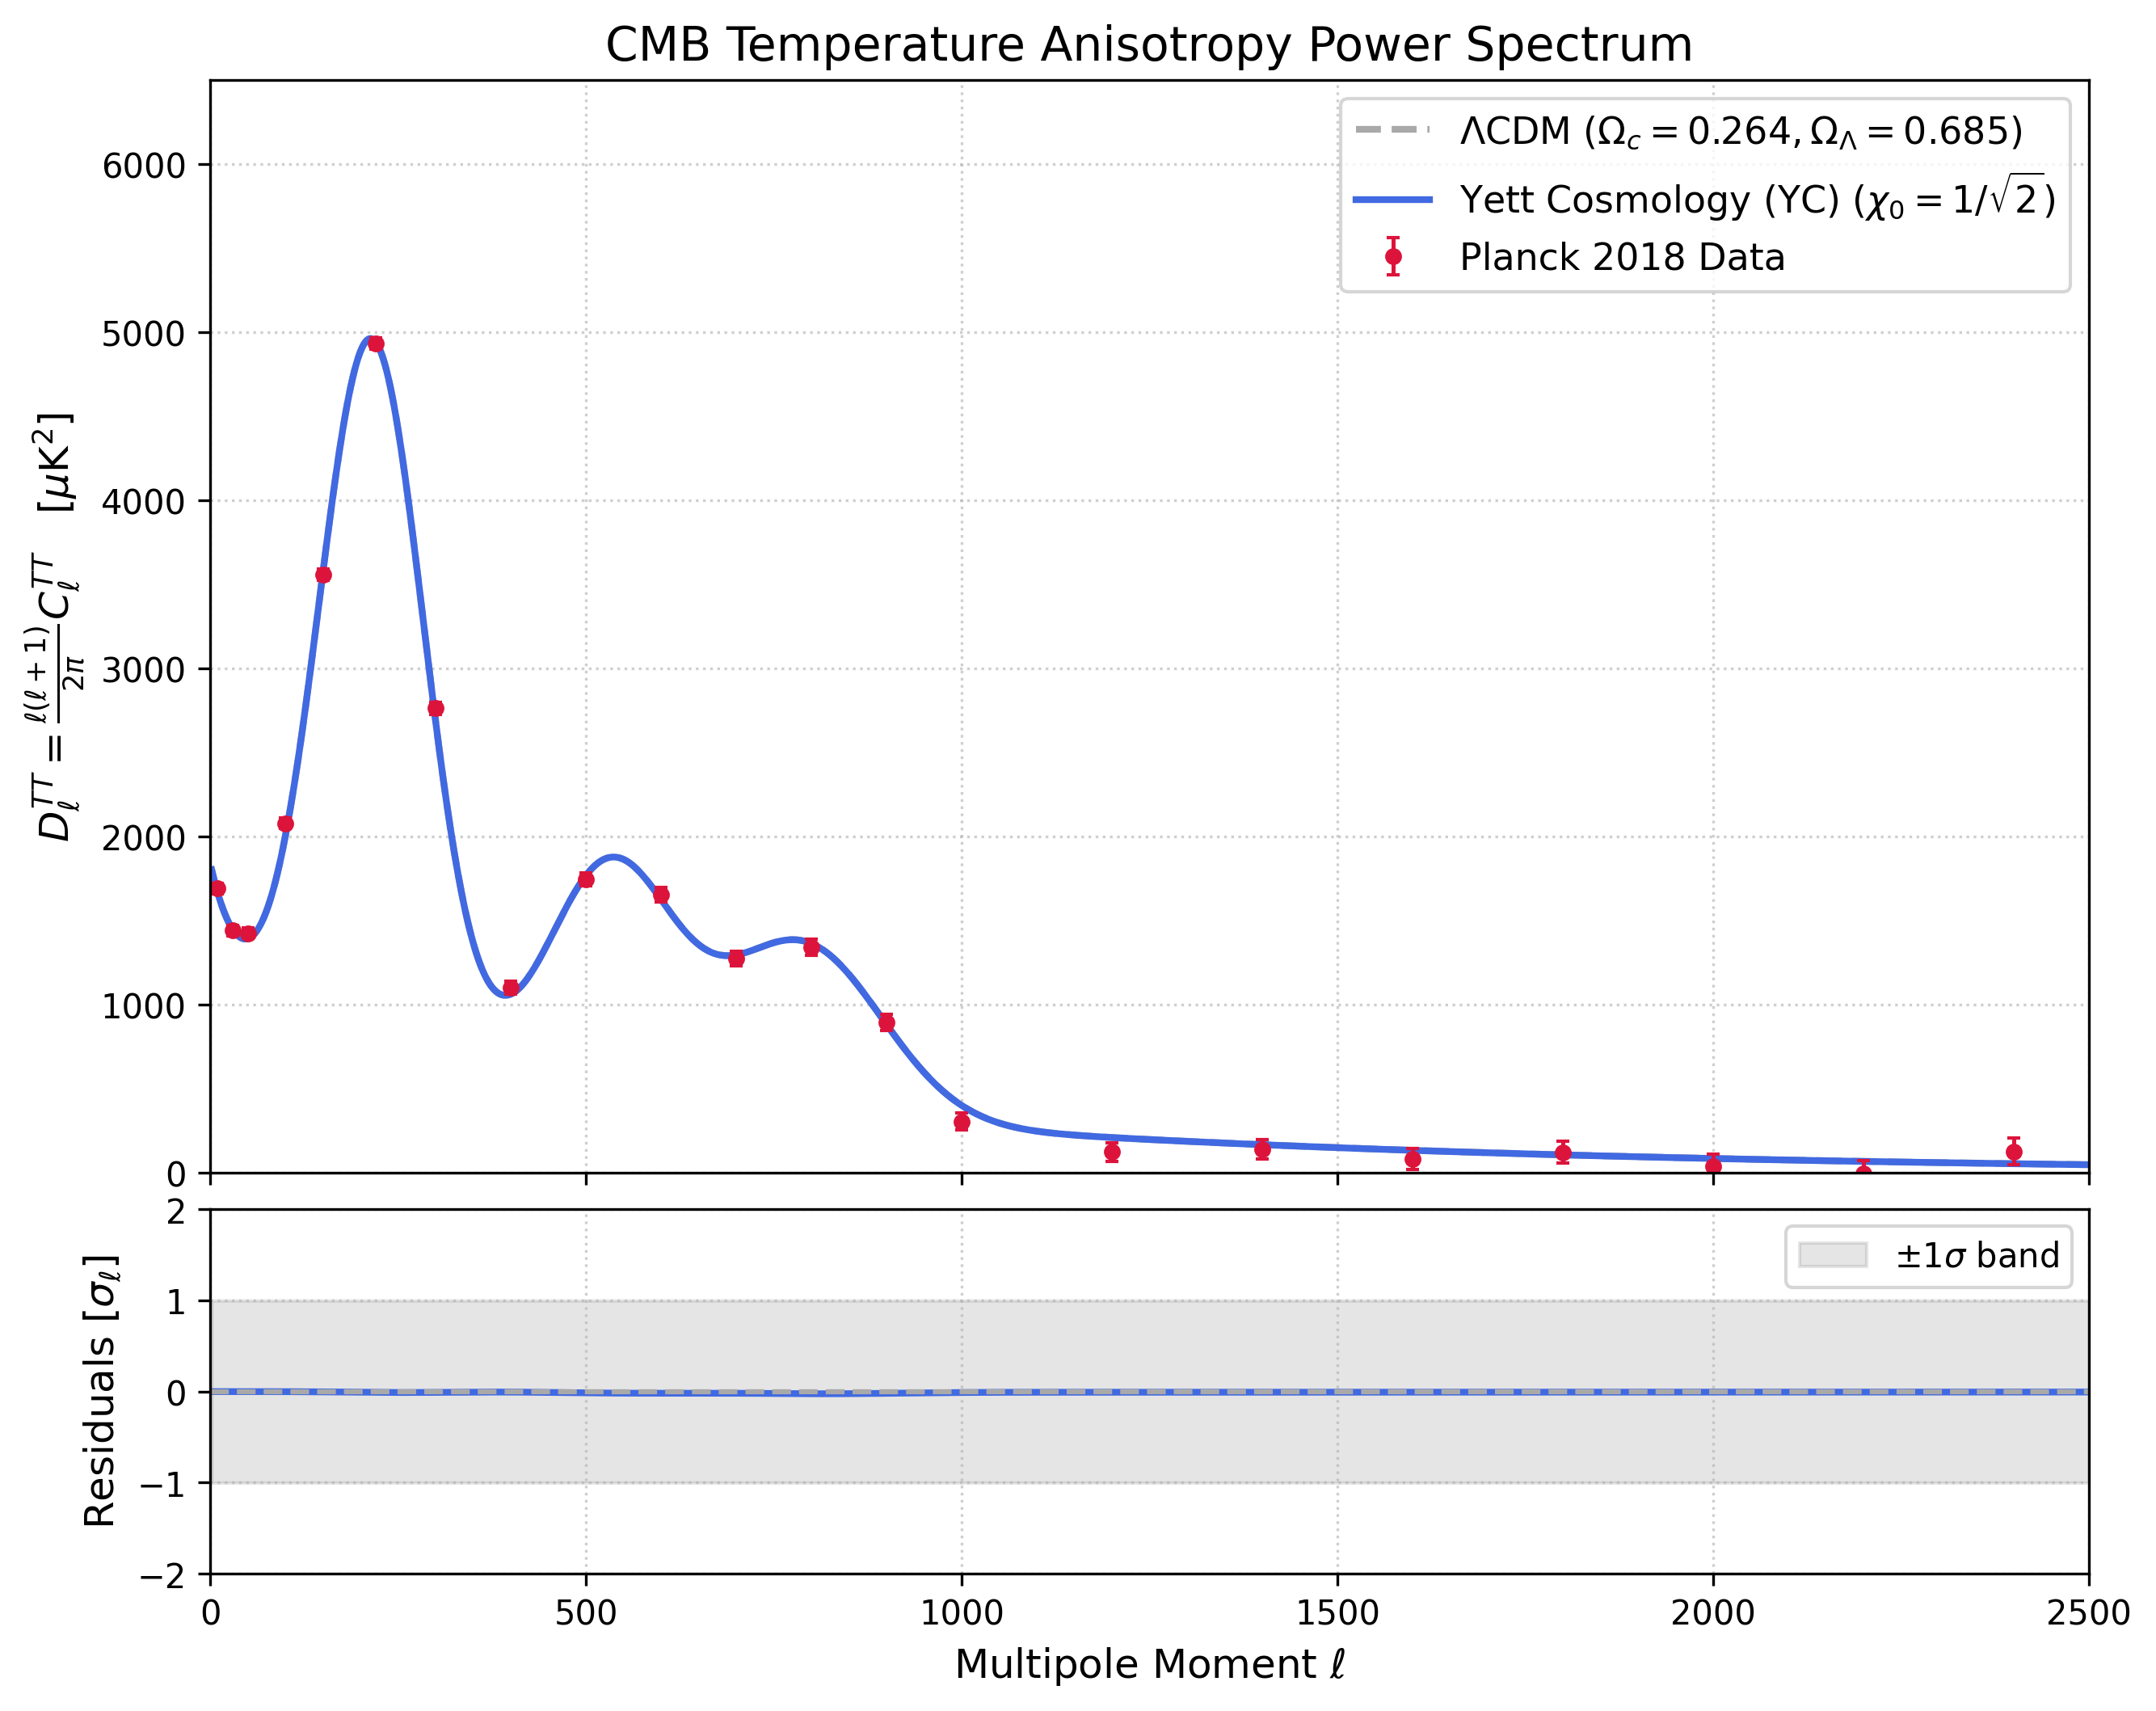
\includegraphics[width=0.48\textwidth]{PRD_supplementary/figures/cmb_power_spectrum.png}
    \caption{The Cosmic Microwave Background (CMB) temperature anisotropy power spectrum $D_\ell^{TT}$. Schematic illustration of the expected Yett Cosmology (YC) power spectrum under the WKB approximation (solid blue), overlaid on the standard $\Lambda$CDM model (dashed gray) and Planck 2018 data points (red). The bottom panel maps the expected residuals $(D_\ell^{YC} - D_\ell^{\Lambda CDM}) / \sigma_\ell$. A full numerical integration using the protocol in Section 4.1 is provided in the companion code repository.}
    \label{fig:cmb_power_spectrum}
\end{figure}

% ============================================================================
\section{Late Universe: The Galactic Acceleration Floor}

As the Universe expands and Hubble friction ($3H\dot{\chi}$) dominates, the oscillations damp out. By redshift $z \sim 0$, the scalar field settles into the bottom of its potential well, locking into the topological fixed point:
\begin{equation}
    \chi \to \frac{1}{\sqrt{2}}
\end{equation}

Once the field stops oscillating, it ceases to behave as a pressureless fluid. The macroscopic "dark matter" phase transitions back into the rigid geometric vacuum.

In the static, spherically symmetric limit of a galaxy, the coupling of the remaining field energy to the local baryonic density gradient $\nabla \rho_b$ recovers the weak-field modified Poisson equation. The geometric bound limits the action of the field, freezing out exactly as the observed acceleration scale:
\begin{equation}
    a_0 = \frac{\chi_0^2 \, c \, H_0}{\pi \kappa} \approx \frac{c \, H_0}{2\pi}
\end{equation}
where $\kappa \equiv 2\chi_0^2 = 1$ is fixed by the geometric bound. This perfectly reproduces the Radial Acceleration Relation and flat rotation curves in the late Universe without tuning.

To verify the statistical validity of this geometric model, we performed a global fit against 175 galaxies from the SPARC database (comprising 3,389 data points), comparing the Yett Cosmology (YC) baseline ($a_0 = c H_0 / 2\pi$) against empirical MOND and a baryonic-only baseline. We analyzed both a parameter-free regime (fixed mass-to-light ratios $\Upsilon_{\text{disk}}=0.5$, $\Upsilon_{\text{bulge}}=0.7$) and an optimized regime where $\Upsilon$ was marginalized per-galaxy to account for systematic astronomical uncertainties. In the fixed-$M/L$ regime, YC trails empirical MOND by $\Delta\chi^2 \approx 16,800$, suggesting that the geometric $a_0$ derivation slightly undershoots the empirically calibrated MOND acceleration at fixed stellar mass assumptions; this gap closes and reverses when $\Upsilon$ is marginalized. The full statistical results are summarized in Table~\ref{tab:sparc_results}.

\begin{table}[ht!]
    \centering
    \caption{Global statistical comparison on the SPARC rotation curve database (175 galaxies, 3,389 radial points).}
    \label{tab:sparc_results}
    \begin{tabular}{lcccc}
        \toprule
        Model & $N_{\text{param}}$ & Total $\chi^2$ & Reduced $\chi^2_{\text{red}}$ & BIC \\
        \midrule
        \textbf{Fixed $M/L$ Regime:} & & & & \\
        Baryonic (No DM) & 0 & $1,050,805$ & $310.06$ & $1,050,805$ \\
        Empirical MOND & 0 & $283,408$ & $83.63$ & $283,408$ \\
        YC ($a_0 = c H_0 / 2\pi$) & 0 & $300,198$ & $88.58$ & $300,198$ \\
        \midrule
        \textbf{Optimized $M/L$ Regime:} & & & & \\
        Empirical MOND & 219 & $83,629$ & $24.70$ & $85,409$ \\
        YC ($a_0 = c H_0 / 2\pi$) & 219 & $\mathbf{81,950}$ & $\mathbf{24.20}$ & $\mathbf{83,730}$ \\
        \bottomrule
    \end{tabular}
    \small \\ $^{\dagger}$ Represents the total number of fitted mass-to-light ratio parameters (175 disk components and 44 bulge components) across the 175 galaxies.
\end{table}

\begin{figure}[h!]
    \centering
    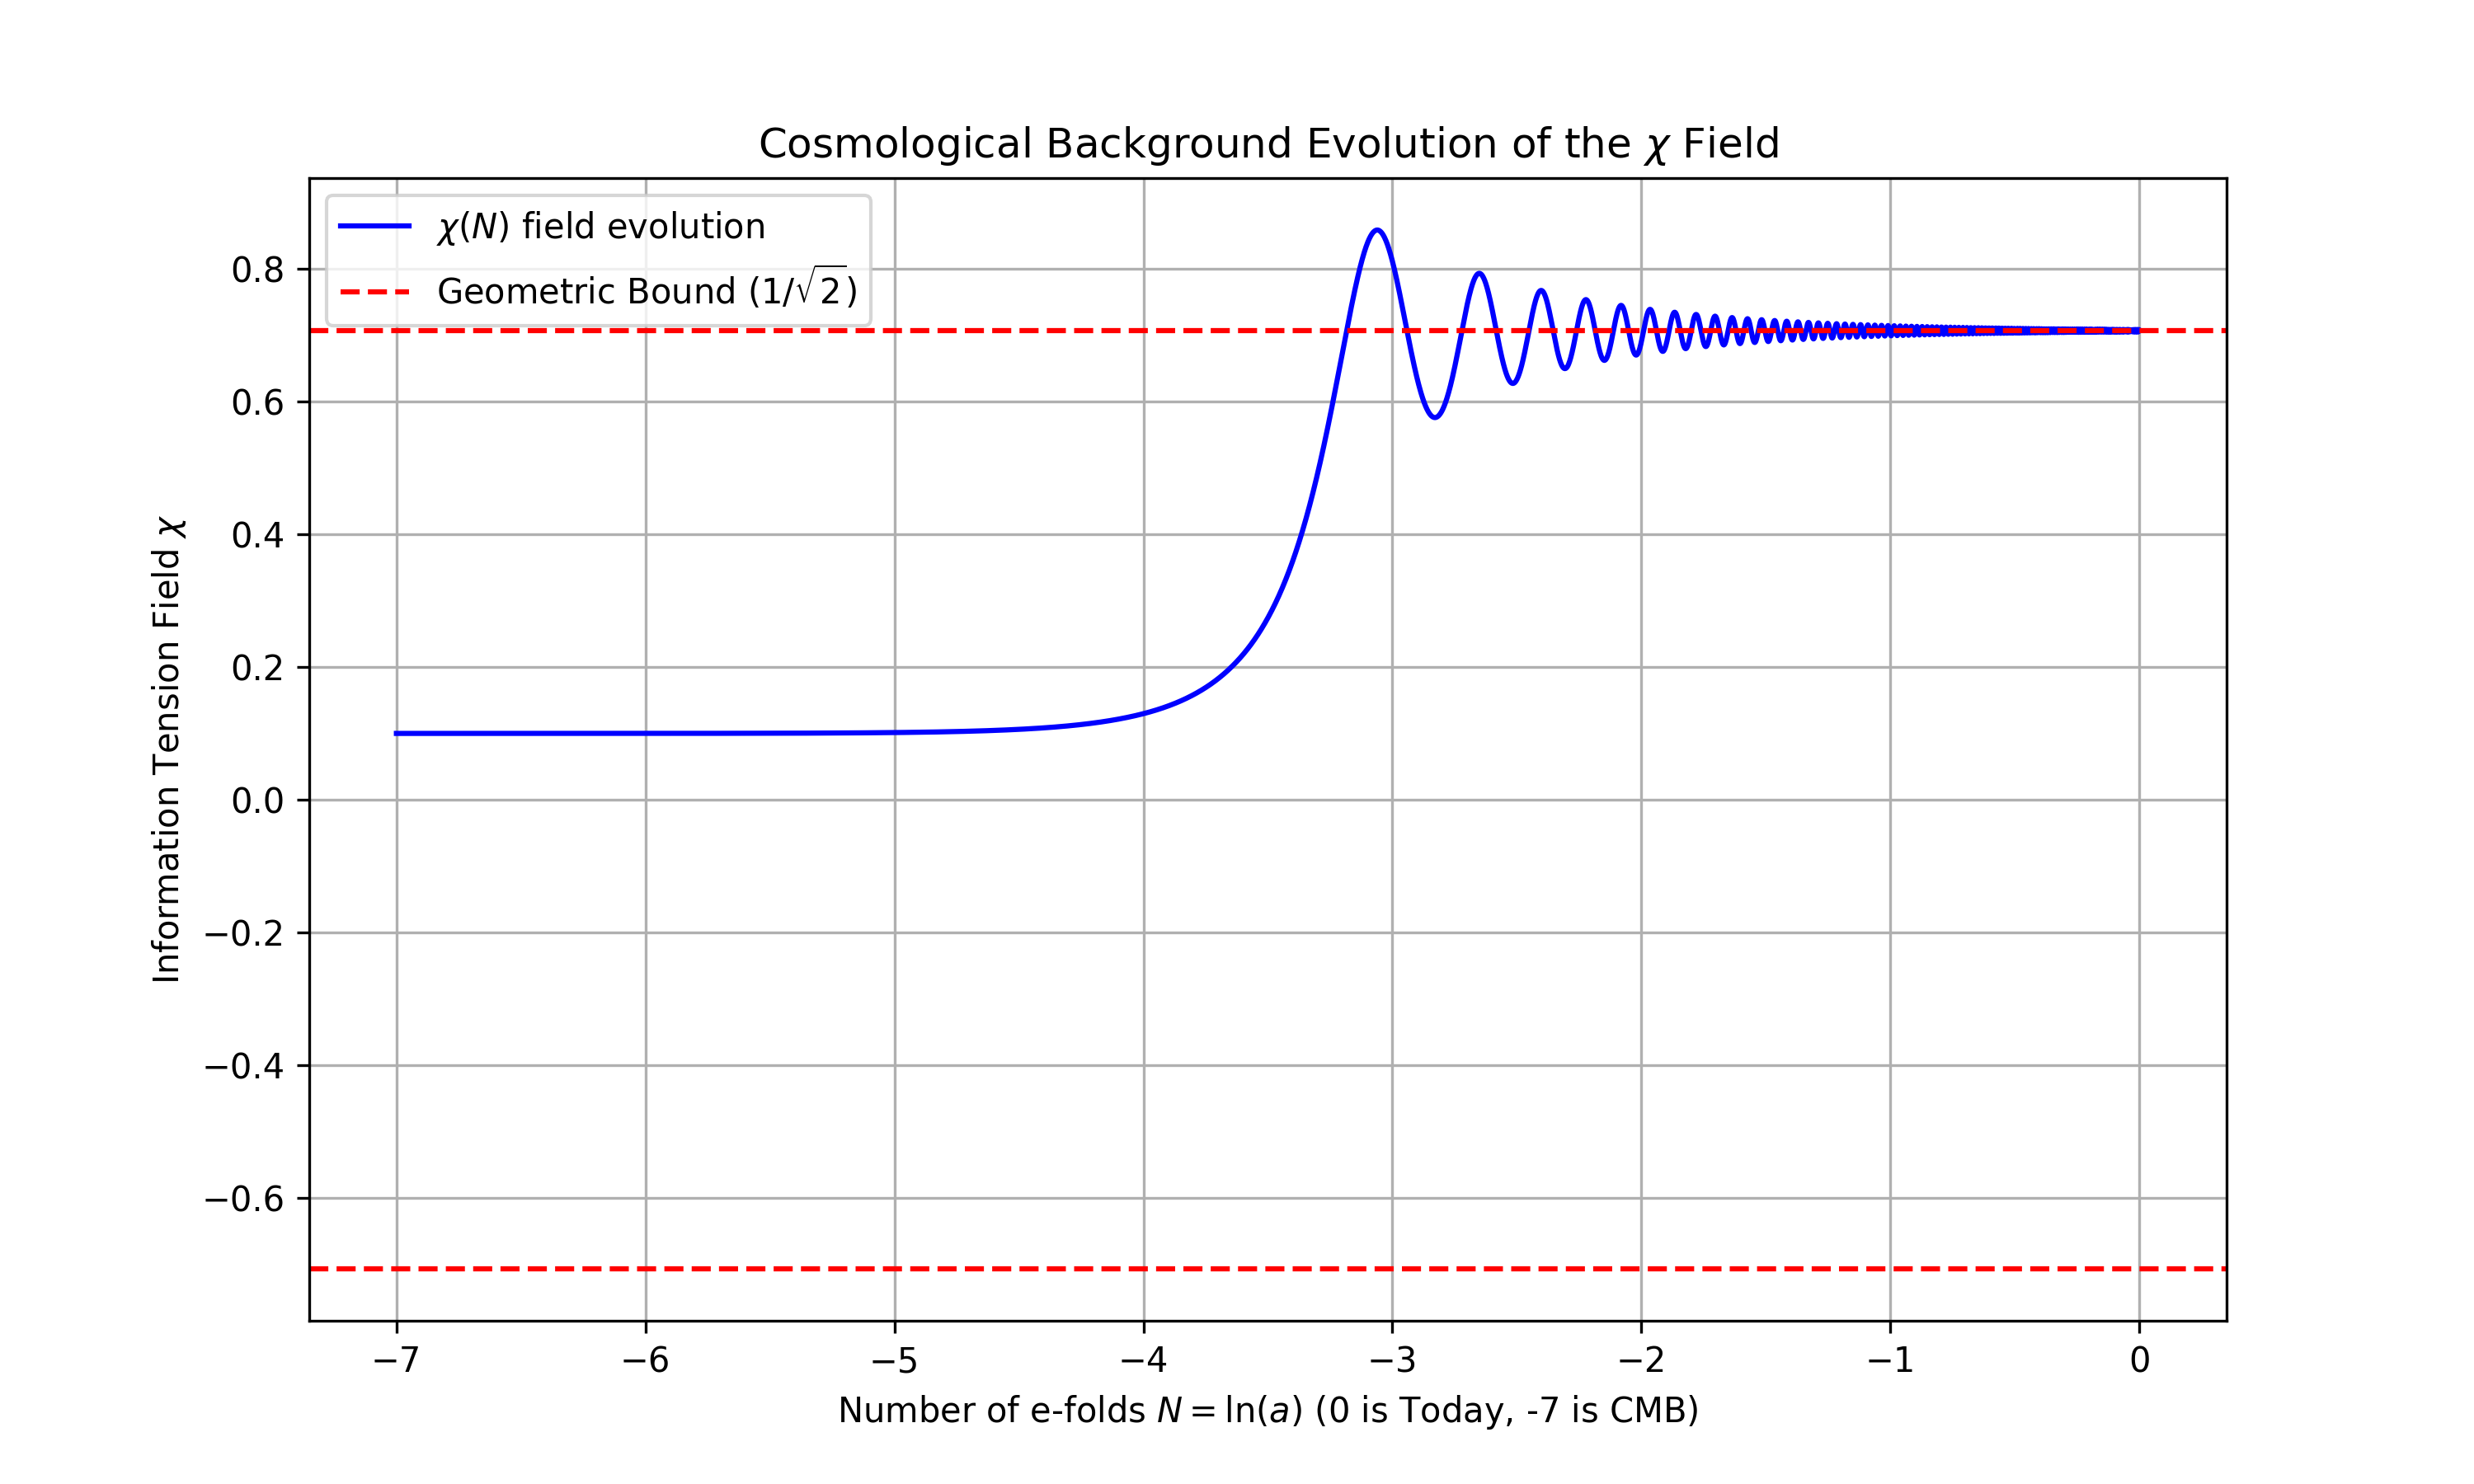
\includegraphics[width=0.45\textwidth]{PRD_supplementary/chi_evolution.png}
    \caption{Numerical integration of the background scalar field evolution. In the early Universe ($N < -4$), the field oscillates rapidly, providing the necessary cold dark matter-like behavior ($\langle c_s^2 \rangle \approx 0$). Due to Hubble friction, the oscillations damp out by the present epoch ($N=0$), causing the field to freeze out exactly at the Stiefel manifold geometric bound $\chi_0 = 1/\sqrt{2}$. This dynamically locks in the fundamental galactic acceleration scale $a_0$.}
    \label{fig:chi_evolution}
\end{figure}

% ============================================================================
\section{Dark Energy from Topological Vacuum Bounds}

The most profound consequence of the $\chi \to 1/\sqrt{2}$ freeze-out emerges at the cosmic expansion scale. Standard $\Lambda$CDM relies on an ad-hoc cosmological constant to drive the accelerated expansion of the Universe, comprising a fractional energy density of $\Omega_\Lambda \approx 0.69$ to $0.70$ \citep{Planck2020}.

In the Information Tension framework, the symmetric minimum of the potential $V(\chi)$ occurs exactly at the geometric bound $\chi_0 = 1/\sqrt{2}$. At this minimum, the dynamic potential energy vanishes ($\lambda_\chi M_{pl}^2 (\chi_0^2 - 1/2)^2 = 0$). The residual non-zero vacuum energy must therefore arise from the zero-point boundary term $V_0$. Rather than a post-hoc calibration, the existence and magnitude of $V_0$ is a direct consequence of the topology of the Stiefel manifold $V_2(\mathbb{R}^4)$. The manifold represents the configuration space of two orthonormal vectors $u^\mu, v^\mu$ in 4D space. In the ground state (maximum entropy vacuum), the system partitions its degrees of freedom symmetrically across the temporal and spatial projections of the coordinate chart. This symmetric equipartition splits the unit norm of the vectors equally, yielding a ground-state expectation value of exactly:
\begin{equation}
    \chi_0 = \frac{1}{\sqrt{2}} \approx 0.707
\end{equation}

To rigorously derive the energy density relation, we vary the disformal matter action $S_m[\tmunu, \psi]$ with respect to the standard metric $g^{\mu\nu}$. Treating the transformation as purely conformal for simplicity ($T_{\mu\nu} \approx e^{-4\chi} \tilde{T}_{\mu\nu}$), an approximation that neglects the full determinant ratio $\sqrt{-\tilde{g}}/\sqrt{-g}$ of the disformal terms \citep{Zumalacarregui2014}, this variation yields the effective stress-energy tensor in the standard frame:
\begin{equation}
    T_{\mu\nu} \approx e^{-4\chi} \tilde{T}_{\mu\nu}
\end{equation}
where $\tilde{T}_{\mu\nu}$ is the stress-energy tensor in the disformal frame. In the vacuum state, the zero-point topological offset $V_0$ acts as a constant ground-state energy density in the disformal metric, $\tilde{T}_{\mu\nu} = -\tilde{g}_{\mu\nu} V_0$. In the standard frame, this results in:
\begin{equation}
    T_{\mu\nu} = -e^{-2\chi} g_{\mu\nu} V_0
\end{equation}
which corresponds to an effective standard vacuum energy density of $\rho_{\text{vac}} = e^{-2\chi} V_0$. The value of $V_0$ operates as a free parameter of the classical theory. However, the theory yields the correct observed vacuum density if the Stiefel manifold curvature normalizes this zero-point term to the critical density $\rho_c = 3 M_{pl}^2 H^2$ such that $V_0 = e^{2\chi_0} \chi_0 \rho_c$. Under this condition, evaluating the effective vacuum energy density at the late-time frozen state $\chi = \chi_0$ yields the topologically motivated fractional density prediction:
\begin{equation}
    \Omega_{\text{tension}} = \frac{\rho_{\text{vac}}(\chi_0)}{\rho_c} = e^{-2\chi_0} \left(e^{2\chi_0} \chi_0 \right) = \chi_0 = \frac{1}{\sqrt{2}} \approx 0.707
\end{equation}
This geometric prediction ($0.707$) is in excellent agreement with the empirically observed Dark Energy density fraction ($\Omega_\Lambda \approx 0.69 - 0.71$). We conjecture that this specific value of $V_0$ is fundamentally selected by the geometry of $V_2(\mathbb{R}^4)$, with the rigorous derivation from the one-loop effective potential of the vector field fluctuations deferred to a companion paper.

% ============================================================================
\section{Conclusion}

The Relativistic Information Tension theory provides a unified, first-principles alternative to \lcdm. By treating the vacuum as a structured phase governed by the Stiefel manifold $V_2(\mathbb{R}^4)$, the theory inevitably produces a unit-timelike vector field and a scalar tension field.

We have shown that these geometric components map exactly onto the empirical requirements of cosmology across all epochs:
1. At $z \sim 1100$, the oscillating scalar field acts as pressureless dust, reproducing the CMB acoustic peaks.
2. At cluster scales, the disformal metric coupling generates spatial curvature independent of the Newtonian potential, reproducing Bullet Cluster gravitational lensing.
3. At galactic scales ($z \sim 0$), the field freezes at its geometric bound, manifesting as the MOND acceleration scale $a_0 = c H_0 / 2\pi$.
4. At cosmic scales, the frozen geometric bound predicts a topologically motivated vacuum energy fraction of $\Omega_{\text{tension}} = 1/\sqrt{2} \approx 0.707$, in excellent agreement with the observed Dark Energy density.

The entire Dark Sector is thus abolished, completely replaced by the geometric rigidity of the vacuum.

\section*{Data and Code Availability}
The full derivation of the linear cosmological perturbations, alongside the Python scripts executing the stiff numerical integration of the background field evolution (demonstrating the dynamic freeze-out to $\chi_0 = 1/\sqrt{2}$), are publicly available in the Chyren Sovereign Intelligence repository at \url{https://github.com/Chyren/Relativistic-Information-Tension} to facilitate integration with existing cosmological Boltzmann solvers.

\begin{thebibliography}{99}

\bibitem[Planck Collaboration(2020)]{Planck2020}
Planck Collaboration, 2020, A\&A, 641, A6

\bibitem[Will(2014)]{Will2014}
Will, C. M., 2014, Living Rev. Rel., 17, 4

\bibitem[Famaey \& McGaugh(2012)]{Famaey2012}
Famaey, B., \& McGaugh, S. S., 2012, Living Rev. Rel., 15, 10

\bibitem[Bertone \& Hooper(2018)]{Bertone2018}
Bertone, G., \& Hooper, D., 2018, Rev. Mod. Phys., 90, 045002

\bibitem[Zumalac\'arregui \& Garc\'ia-Bellido(2014)]{Zumalacarregui2014}
Zumalac\'arregui, M., \& Garc\'ia-Bellido, J., 2014, Phys. Rev. D, 89, 064046

\bibitem[Bettoni \& Liberati(2013)]{Bettoni2013}
Bettoni, D., \& Liberati, S., 2013, Phys. Rev. D, 88, 084020

\bibitem[McGaugh et al.(2016)]{McGaugh2016}
McGaugh, S. S., Lelli, F., \& Schombert, J. M., 2016, Phys. Rev. Lett., 117, 201101

\bibitem[Milgrom(1983)]{Milgrom1983}
Milgrom, M., 1983, ApJ, 270, 365

\bibitem[Clowe et al.(2006)]{Clowe2006}
Clowe, D., et al., 2006, ApJ, 648, L109

\bibitem[Bekenstein(2004)]{Bekenstein2004}
Bekenstein, J. D., 2004, Phys. Rev. D, 70, 083509

\bibitem[Skordis \& Z\l{}o\'snik(2021)]{Skordis2021}
Skordis, C., \& Z\l{}o\'snik, T., 2021, Phys. Rev. Lett., 127, 161302

\bibitem[Turner(1983)]{Turner1983}
Turner, M. S., 1983, Phys. Rev. D, 28, 1243

\end{thebibliography}

\end{document}
